\documentclass[11pt]{article}
\usepackage{geometry}                
\geometry{letterpaper}                   

\usepackage{listings}
\usepackage{graphicx}
\usepackage{epstopdf}
\usepackage{varioref}
\usepackage[numbers]{natbib}
\usepackage[squaren]{SIunits}
\usepackage{amssymb, amsmath}
\DeclareGraphicsRule{.tif}{png}{.png}{`convert #1 `dirname #1`/`basename #1 .tif`.png}

\title{Modelling Situations of Evacuation in a Multi-level Building}
\author{Hans Hardmeier, Andrin Jenal, Beat Küng & Felix Thaler}
\date{date} 

\begin{document}



\thispagestyle{empty}

\begin{center}

\includegraphics[width=5cm]{ETHlogo.eps}

\bigskip


\bigskip


\bigskip


\LARGE{ 	Lecture with Computer Exercises:\\ }
\LARGE{ Modelling and Simulating Social Systems with MATLAB\\}

\bigskip

\bigskip

\small{Project Report}\\

\bigskip

\bigskip

\bigskip

\bigskip


\begin{tabular}{|c|}
\hline
\\
\textbf{\LARGE{Insert Title Here}}\\
\textbf{\LARGE{...}}\\
\\
\hline
\end{tabular}
\bigskip

\bigskip

\bigskip

\LARGE{Name 1 \& Name 2}



\bigskip

\bigskip

\bigskip

\bigskip

\bigskip

\bigskip

\bigskip

\bigskip

Zurich\\
March 2012\\

\end{center}



\newpage

%%%%%%%%%%%%%%%%%%%%%%%%%%%%%%%%%%%%%%%%%%%%%%%%%

\newpage
\section*{Agreement for free-download}
\bigskip


\bigskip


\large We hereby agree to make our source code for this project freely available for download from the web pages of the SOMS chair. Furthermore, we assure that all source code is written by ourselves and is not violating any copyright restrictions.

\begin{center}

\bigskip
\bigskip
\bigskip
\bigskip


\begin{tabular}{@{}p{3.3cm}@{}p{6cm}@{}@{}p{6cm}@{}}

\begin{minipage}{3cm}

\end{minipage}
&
\begin{minipage}{6cm}
\vspace{2mm} \large Hans Hardmeier

 \vspace{\baselineskip}

\end{minipage}
&
\begin{minipage}{6cm}

\large Andrin Jenal

\end{minipage}

\end{tabular}

\bigskip
\bigskip
\bigskip
\bigskip


\begin{tabular}{@{}p{3.3cm}@{}p{6cm}@{}@{}p{6cm}@{}}

\begin{minipage}{3cm}

\end{minipage}
&
\begin{minipage}{6cm}
\vspace{2mm} \large Beat Küng

 \vspace{\baselineskip}

\end{minipage}
&
\begin{minipage}{6cm}

\large Felix Thaler

\end{minipage}
\end{tabular}

\end{center}
\newpage

%%%%%%%%%%%%%%%%%%%%%%%%%%%%%%%%%%%%%%%



% IMPORTANT
% you MUST include the ETH declaration of originality here; it is available for download on the course website or at http://www.ethz.ch/faculty/exams/plagiarism/index_EN; it can be printed as pdf and should be filled out in handwriting

%TODO: The is declaration of originality on the WEb for Windows (Andrin Jenal)...

%%%%%%%%%% Table of content %%%%%%%%%%%%%%%%%

\tableofcontents

\newpage

%%%%%%%%%%%%%%%%%%%%%%%%%%%%%%%%%%%%%%%



\section{Abstract}

If you are an ETH-Student, you know that at lunch time it is almost impossible to go out of the building through the main entrance to the polyterasse, because of the number of students trying to leave at the same time. What would happen, if in addition to that, a panic factor was involved? Have you ever imagined, how an evacuation at the ETH Main building, ETH CAB-Building or even at your own home would look like? How many people would be able to leave simultaneously? What is the best strategy for people to leave? How would the perfect evacuation plan for your school or enterprise building look like?

In this work, we decided to elaborate a program that is flexible enough to calculate the best evacuation-scenario for every given structure. Using the "Fast Sweeping Algorithm Method", introduced by James A. Sethian\cite{Zhao04afast} to solve this complex problem involving physical forces and psychological reactions, MATLAB is capable of computing the most efficient way for every agent (person) to leave a given multi-floor map.

Different from all other similar projects, we also focused on an efficient and realistic implementation of the program. Coding our own data structures to handle with the numerous amount of agents, implementing the "Fast Weeping Algorithm Method" in such way that MATLAB takes advantage of it and also counting with all details of the human behavior while moving/running, this work introduces a tool to verify the potential of evacuation in any given structure.


\section{Individual contributions}


.....

On the other hand Carl Hans Peter Hardmeier Samame, alias Hans Hardmeier, was responsible for some parts of the documentation, verification of the MATLAB-code and calculating efficienty using different operating systems (i.e. Mac OS 10.6).


%TODO: Wer het was gmacht... (Jede : Beat, Hans, Andrin, Felix)

\section{Introduction and Motivations}

\subsection{Introduction}

Simulating the evacuation scenario of a single-level building is well known but is not general enough. Though we want to introduce a more sophisticated simulation within a multi-level building. E.g.: What would happen, if a multi-level building has to be evacuated? Which escape routes would be mostly used? Which effects would have the pressure/panic of other persons into the situation? Since tower buildings are getting more common in large cities, engineers have to care more about the behaviour in situations of emergency, namely evacuations. Apart of the mathematical model and implementation for solving this problem, we also wanted to increase the utility of this program for all readers by giving the possibility of calculate different scenarios in different buildings given by the user. In this work, we will work with the map of the ETH building, however, it is to notice that you can replace any map with others that meet the properties of the Figure \ref{building floor image} in the section \ref{matlab code}.

\subsection{Motivation}

Intuitive expectations and mathematical model results can stay sometimes in contradiction. As ETH-Students is for us the safety of the people inside the ETH Mainbuilding very important. But on the one hand, we are know sure, if the evacuation potential of the building is enough for the amount of students during a normal week day and on the other hand, we want to help the people around the world, that have a similar question, to find an answer. This two points gave us the ideas and motivation to create a flexible tool that simulates a real-world scenario for any given building or even structures (i.e. planes or boats).

\subsection{Fundamental Questions}

\begin{enumerate}
\item Which places in a building do contribute the crucial part to panic behaviour?
\item Do the results correspond to the literature? Why? - Why not?
\item What are the similarities to single level evacuation bottleneck?
\item What are the most influential forces, which decide the behavior of scenario?


\end{enumerate}


\section{Description of the Model}

%TODO: finalize (write out every etc.) Hans compare with RESEARCH! -> Froge zerscht (Beim Introduction)und ausschreiben
% TODO MERGE WITH RESEARCH!!! Andrin Jenal

To investigate it, we will create a relatively general framework for behavioral simulation in evacuation scenarios. That includes every non-trivial, relevant force affecting every agent i.e. repulsion within the agents (unconscious privacy area conservation), detection of environment (walls, exits, stairs - inclusive direction-, evtl. source of evacuation,etc ) rational thinking to calculate the way to exit (run-time calculation with fast-sweeping algorithm), etc.


\subsection{General Model}

We are planning to base our work on the social force model \cite{SFMPD}. The  behaviour of the agents will be mainly influenced by different model parameters like obstacles, stairs and other agents. In addition, psychological pressure in such evacuation scenarios are going to be investigated. The following points are the chosen parameters for the model in this work. For more precisely mathematical explanations, see \cite{SFMPD}




\subsection*{Agents Repultion Force}

Within a evacuation scenario, the psychological tendency of two pedestrians i and j to stay away from each other, depends on the level of repultion between this two specific agents (margin of unconscious privacy area conservation between them). In addition, we assume two other more physical forces: a `body force' counteracting body compression (important factor in a panic evacuation model) and a `sliding friction force' avoiding the unnatural regulation of the speed when the agent nears another. 

\subsection*{Physical Objects}

Using the nearest point in a wall to an agent, the repulsive forces created by the whole wall is treaten analog as the created Agents-Repultion-Forces. At the same time, the preprocessing of the map, together with the exits and stairs, allows us to create a gradient field all over the map, that shows the agent, the shortest way to exit the floor. 

%%Evtl.  example of field force?? from /images


\subsection*{Force of Agents}

Quote from 'Helbling, Dirk - Molnar, Peter (1995): Social Force Model for Pedestrians Dynamics' \cite{SFMPD} :

\textit{"The desired velocity $v^0_i$ can reach more than $5 \meter\second^{-1}$ (up to $10 \meter\second^{-1}$), but the observed free velocities	for	leaving	a	room	correspond	to	$v^0_i=6 \meter\second^{-1}$ under relaxed, $1\meter\second^{-1}$ under normal, and $1.5\meter\second^{-1}$ under nervous conditions. A reasonable estimate for the acceleration time is $0.5\meter\second^{-1}$."}

In our model, although the mass is not visible, it is from enorm importance for the calculation of the force of each agent. It's well known that the inertia of each agent is directly dependent from his mass and velocity..



\subsection{Research}

The core investigation is a szenario which describes the panic behaviour of individuals in a crowded building. Whereas at the beginning of each simulation the setting is a general everyday situation and at the end we should be able to make strong statements anwsering our fundamental questions.
Relying on a fairly recent paper [Halbling2000] we tried to get our simulation as accurate to reality as possible. Since this model is based on above mentioned forces and interactions we tried to figure out how agents overcome major obstacles like tiny passages and stairs. Here the shape of rooms and building is a key factor contributing to the behaviour of agents.
Therefore we defined a special setting concerning agents on stairs, which includes reduces velocity.

% TODO: ausführlicher
As a core investigation we are going to simulate an everyday situation in a crowded (public) environment ending in an evacuation scenario.





\section{Implementation}
Our goal was a fast implementation of the model. So we decided to use the Fast
Sweeping algorithm instead of the Fast Marching alorithm to calculate the
fastest way out of a building. We knew that \textit{MATLAB} code is not very fast and
\textit{MATLAB} provides an interface for other programming languages. So we
used \textit{C} to
implement the Fast Sweeping method.

Later in the development process we discovered another bottleneck in our code:
The social force between the agents which runs in $ O(N^2) $. Felix then
introduced a Range Tree for this problem, which he also implemented in
\textit{C}.

\subsection{\textit{MATLAB} Code} \label{matlab code}
We wanted to create a flexibel model which can be used to simulate every
possible building structure. 

Each scenario is described in a config file. This includes for example how many
agents are placed on each floor or the timestep of the simulation (the exact
definition can be found in the file data/config\_file\_structure). Each config
file also references one or more building floor images.
Figure \vref{building floor image} describes how a building floor
image must look like. The agents are placed randomly within the agents spawning
area(s).

\begin{figure}[h]
\centering
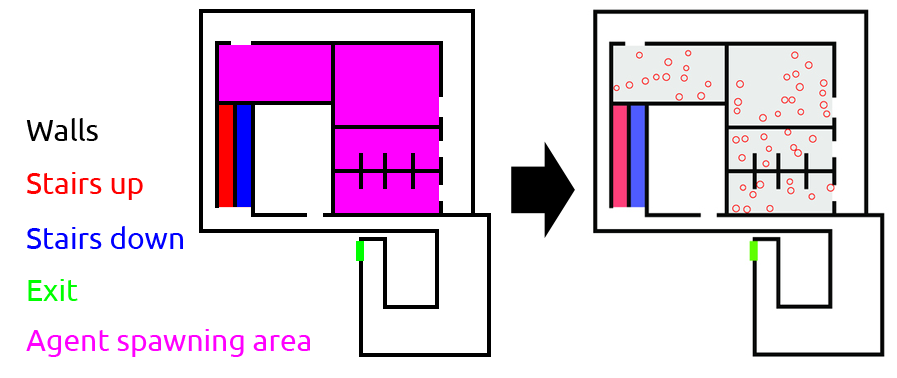
\includegraphics[width=\textwidth]{config_floor_description.png}
\caption{Left the building floor image and right how it looks when the
simulation is running} 
\label{building floor image}
\end{figure}

Since \textit{MATLAB} is not really object-oriented, we used a big data structure (called
data) that includes all internal data that we use (eg. the floors and agents).
It is passed as an argument for every function that needs it.

\subsection{Pathfinding}
As described in \cite{SFMPD}, the agents always try to reach their desired destination using the shortest possible path. As we use raster graphics to encode simulation data, we decided to use the same discrete grid to compute the nearest path to an exit for every point approximately.
Mathematically, this can be expressed as an partial differential equation, the 2D Eikonal equation (equation \ref{eq:eikonal}).

\begin{equation} \label{eq:eikonal}
\|\mathbf{\nabla} d(\mathbf{x})\|=1 \quad d:\!\mathbb{R}^{2}\to\mathbb{R},\mathbf{x}\in\mathbb{R}^{2}
\end{equation}

The solution $d(\mathbf{x})$ now gives the distance to the nearest exit point, its negative gradient $-\mathbf{\nabla}d(\mathbf{x})$ therefor always points in the direction of the shortest path towards the desired exit. There are mainly two competitive agorithms for solving this equation efficiently. First there is the \textit{Fast Marching} method, a specialized version of Dijkstra's well known algorithm \cite{dijkstra59a}. The alternative is \textit{Fast Sweeping}, which leads to a much simpler implementation, faster calculation and better algorithmic complexity of $O(n)$ instead of $O(n\log n)$ with respect to the discretization size. We therefor implemented an efficient \textit{Fast Sweeping} method, closly following \cite{Zhao04afast} as a basis of our pathfinding and repulsive wall forces. The algorithm uses an upwind finite difference scheme where our mesh is defined by the input images. The implementation was done \textit{C} and not directly in \textit{MATLAB}, using optimized boundary condition handling for our pruposes. Our benchmarks showed a high speed increase compared to other Eikonal solvers, e.g. the "Accurate Fast Marching" implementation as found at \textit{MATLAB CENTRAL} \cite{fastmarching}.

\subsection{Range Tree}
The most time consuming part in our program is the calculation of the interaction forces between the agents, at least if their count is high enough. To reducue the natural complexity of $O(n^{2})$ of this inter-agent interaction, we can clamp forces with little effect, e.g. in our implementation all forces smaller than $ 10^{4}\newton$. As their exponentially decreasing, the distance in which the forces need to be adressed is only several meters, so a big part of them can just be ignored without introducing a significant error.
To get all agents influenced by another agent, we need to be able to search neighbours of any agent within a given distance. To efficiently query these agents, we implemented a 2D range tree in \textit{C}, which allows query times of $O(\log n+k)$, where $n$ is the total number of agents and $k$ is the number of queried agents \cite{algdat}. In larger simulations this reduces simulation times by a significant factor.


\subsection{Profiling \& optimization}


%TODO: 
% profiler resultat diskutieren
%  addAgentRepulsiveForce langsam, da N^2
%  interp2: konstante funk., nicht schneller mit '*nearest', viel langsamer mit (lerp2 schneller...) (Hans)
%  'linear'  

Using the \textit{Profiler}-function of \textit{MATLAB}, we were able to discuss the efficiency of our implementation. The following image show the time comsumption for the calculation of the evacuation of 200000 floors within 15000000 secounds: %%TODO:Only example und ausführlicher, neu runne

\medskip

\begin{center}
	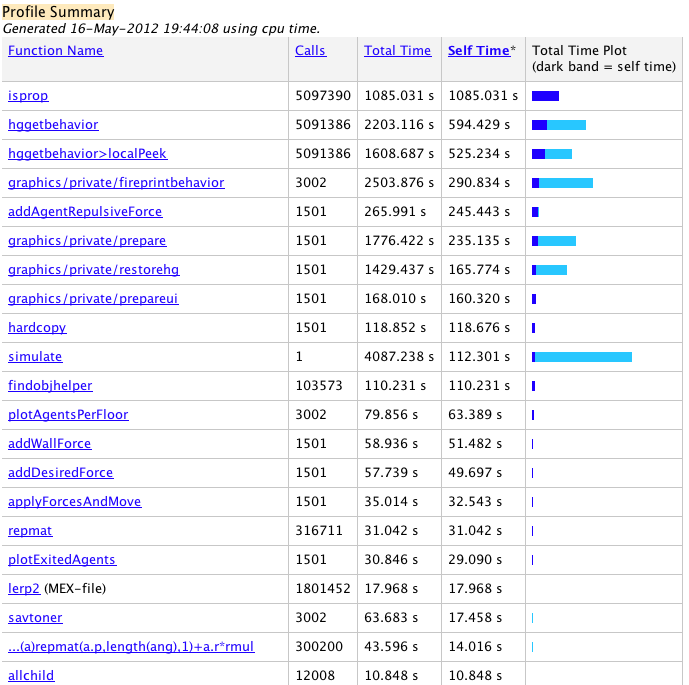
\includegraphics[width=0.9\textwidth]{./images/profiler.png}
\end{center}

We tried to optimize the code using the parallel for-loop parfor in \textit{MATLAB}. In
the function applyForcesAndMove we replaced the for-loop over the agents with
parfor. We measured the time using an input with 200 agents on a 4 core machine
using 5 \textit{MATLAB} workers. The result was that the parfor version was even slightly
slower than the serial version. The reason for this is how \textit{MATLAB} implements
parfor: all the memory that is used by a worker must be sent to this worker.
Each agent must access the building floor image randomly and this creates a
large amount of memory that must be transferred to each worker, which leads to a
decreasing performance.
This is why we decided not to use parfor or any other parallelization in our
implementation.

\section{Simulation Results and Discussion}

\subsection{Expected Results}

We expect the stairs and the main building exit to be the bottlenecks. The amount of people in lower levels is increasing with time until a certain point, when most of the people have exited the building. Also we think that if the speed (velocity) of the people is higher (people are more in panic), jams at the exit will increase and people will mainly try to take the main exit instead of emergency exits.

\subsection{Simulation Results}

%TODO: add some plots, ...

\subsection{Discussion}


\section{Summary and Outlook}

In this section we would like to thank the MSSSM-Group from the ETH in Zurich, Switzerland directed by Karsten Donnay and Stefano Balietti for their engagement in the lecture "Modeling and Simulating Social Systems with \textit{MATLAB}" during the Spring Semester 2012.


%TODO: Rückblick aufs projekt & Danksagung

\section{References}

\begin{thebibliography} {9}
	
	\bibitem{Zhao04afast} Zhao, Hongkai (2004): A Fast Sweeping Method for Eikonal Equations.
	\bibitem{SFMPD} Helbling, Dirk - Molnar, Peter (1995): Social Force Model for Pedestrians Dynamics.
	\bibitem{AACIBF} Helbling, Dirk, Johansson, Anders (2006): Analytical Approach to Continuous and Intermittent Bottleneck Flows.
	\bibitem{ACPPD} Schadschneider, Andreas et al. (2002): CA Approach to Collective Phenomena in Pedestrian Dynamics.	
	\bibitem{DCD} Helbling, Dirk, Johansson, Anders (2007): Dynamics of crowd disasters: An empirical Study.
	\bibitem{SDFEP} Helbling, Dirk et al. (2000): Simulating dynamical features of escape panic.
	\bibitem{SPCD} Helbling, Dirk et al. (2005): Self-Organized Pedestrian Crowd Dynamics: Experiments, Simulations, and Design Solutions.
	\bibitem{dijkstra59a} Dijkstra, Edsger W. (1959): A Note on Two Problems in Connexion with Graphs.
	\bibitem{fastmarching} Kroon, Dirk-Jan (2011): http://www.mathworks.com/matlabcentral/fileexchange/24531-accurate-fast-marching
	\bibitem{algdat} Ottmann, Thomas, Widmayer, Peter (2002): Algorithmen und Datenstrukturen, 4. Auflage.

\end{thebibliography}

% use \cite{SFMPD} for citation

\section{Appendix}

\subsection{Code}

%TODO: (Felix) Format of Code
\lstset{language=Matlab,breaklines=true}

\lstinputlisting[caption=simulate.m]{../code/simulate.m}
\lstinputlisting[caption=plotFloor.m]{../code/plotFloor.m}
\lstinputlisting[caption=plotExitedAgents.m]{../code/plotExitedAgents.m}
\lstinputlisting[caption=loadConfig.m]{../code/loadConfig.m}
\lstinputlisting[caption=initWallForces.m]{../code/initWallForces.m}
\lstinputlisting[caption=initialize.m]{../code/initialize.m}
\lstinputlisting[caption=initEscapeRoutes.m]{../code/initEscapeRoutes.m}
\lstinputlisting[caption=initAgents.m]{../code/initAgents.m}
\lstinputlisting[language=C,caption=getNormalizedGradient.c]{../code/getNormalizedGradient.c}
\lstinputlisting[language=C,caption=fastSweeping.c]{../code/fastSweeping.c}
\lstinputlisting[caption=checkForIntersection.m]{../code/checkForIntersection.m}
\lstinputlisting[caption=applyForcesAndMove.m]{../code/applyForcesAndMove.m}
\lstinputlisting[caption=addWallForce.m]{../code/addWallForce.m}
\lstinputlisting[caption=addDesiredForce.m]{../code/addDesiredForce.m}
\lstinputlisting[caption=addAgentRepulsiveForce.m]{../code/addAgentRepulsiveForce.m}

%TODO: Add all code-files

\end{document}  



 
